\documentclass[a4paper, 12pt]{article}
\usepackage{matnoble-doc-en}


\begin{document}

\title{\bf {CHEM400/740: Quantum Mechanics in Chemistry}} \author{\bf
  \href{http://scienide2.uwaterloo.ca/~nooijen/website_new_20_10_2011/About.html}{Marcel Nooijen}} \date{}
  
\pagestyle{fancy} \fancyhead[L]{\textcolor{PrimaryColor}{CHEM400/740: Quantum Mechanics in Chemistry}} \fancyhead[R]{\textcolor{PrimaryColor}{2021 Winter}}


\maketitle
\tableofcontents

\footnote{\noindent \createtext{January 16, 2021} \newline
  \updatetext{\today}\newline Edited by: Nan Song}.

\clearpage

\section{Syllabus}
Lectures: \qquad Tuesday \& Thursday \qquad  10:00-11:20 AM\qquad  Microsoft Teams Meeting \newline

\indent Website: \qquad \href{http://scienide2.uwaterloo.ca/~nooijen/website_new_20_10_2011/440F.html}{CHEM400/740 Website Link}\newline

\indent Text Book:\quad   “Modern Quantum Chemistry” by Szabo and Ostlund \newline
\indent \qquad  \qquad \qquad  ISBN: 978-0486691862 \newline
\indent \qquad  \qquad \qquad  More reading material will be provided as the course continues and can be found \indent \qquad  \qquad \qquad  on the class website. \newline

\indent Grading: \qquad The course will have extensive assignments that will be graded.\newline
\indent \qquad  \qquad \qquad  6 Writing Assignments + 3 Python Assignments/ Literature Review\newline
\indent \qquad  \qquad \qquad For grad students, program assignments are mandatory.\newline
\indent \qquad  \qquad \qquad  Also, Students are encouraged to collaborate on assignments. \newline 
\indent \qquad  \qquad \qquad There will not be a midterm or final exam.



\subsection{Description}
In the winter 2021 term the prime focus of the course will be electronic structure theory (70-80\%). A second topic will concern vibronic theory, going beyond the Born-Oppenheimer approximation. The course will cover a description of the basic electronic structure problem introducing an atomic orbital basis set, Slater determinants and the Slater-Condon rules. Then we will cover Hartree-Fock theory in fair detail, and discuss the fundamentals of Density Functional Theory. In a next part of the course I will discuss vibrations and the use of vibronic models. We will discuss second quantization for bosonic operators, and the DVR technique to solve for vibronic eigenstates. Next we will move on to the technique of second quantization for Fermions and discuss techniques to include electron correlation: Configuration Interaction, Coupled Cluster, methods for excited states. Second quantized methods, Wick’s theorem and (perhaps) diagrammatic techniques will be discussed. It is my intention that students will write their own (simple) programs to do actual calculations: a) Hartree-Fock; b) Vibrational / Vibronic calculations; c) CI calculations. If students have very little programming experience they can opt to do a literature review project.

\subsection{Outline of Topics to be Covered}
\begin{itemize}
    \item[ A)] The electronic structure problem: 
    the finite basis full CI model of quantum chemistry.
    
    CI (Configuration Interaction): Exact Schr{\"o}dinger solution in a finite basis set. \fbox{Conceptual mostly!}

    \item[ B)] Discussion on symmetry and spin permutational symmetry.
    
    
    \item[ C)] Slater rules for matrix-elements. 
    
    Solving model problems for atoms.
    \item[ D)] Hartree-Fock (HF) Theory.
    
    Density Functional Theory (DFT).
    \item[ E)] Second quantization:\newline
	- Operator solution for Harmonic oscillator (Bosons).
    \indent eg, ladder operators \newline
    - Occupation number representation for electrons.\newline
    - Second quantized form of $\hat{H}$.
    \item[ F)] Deriving equations using second quantization:\newline
    - CI single for excited states.\newline
    - CI double for ground states.
    \item[ G)] Normal order and Wick's theorem. (Some diagrammatic techniques)
    \item[ H)] Using second quantization to discuss:\newline
    - Configuration Interaction.\newline
    - Coupled Cluster (CC) Theory. \newline
    - CC method for excited states. (The equation of motion CC to get excited states)\newline
    - Analytical energy derivative and density matrices.
    \item[ I)] Contemporary topics in quantum chemistry:\newline
    - Local correlation. \newline
    - Explicit Correlation. \newline   
\end{itemize}


\section{Review Session}

\subsection{Dirac Bra-ket Notation}
Typically in quantum mechanics, the bra-ket notation represents a state of quantum system. The notation uses the angle brackets, ``$\langle$" and ``$\rangle$", and a vertical bar ``|".\\
\indent In a specific quantum state $\psi(r_1,r_2,...,r_N)$, ket is a symbol that has a straight bar and a angle to represent quantum state. eg, $|\psi\rangle$.
\paragraph{Ket Notation}~{}\\
\indent The operator $\hat{A}$ acts on a state $| a_i\rangle$. It can be written as:
\begin{equation}
\hat{A}| a_i\rangle = a_i| a_i\rangle  
\end{equation}
\begin{itemize}
\item $\hat{A}$ is an operator. eg, the position operator $\hat{x}$, and the momentum operator $\hat{p}_x$. 
\item $a_i$ is an eigenvalue (just a number). 
\item $|a_i\rangle$ is an abstract representation for eigenstate of the operator $\hat{A}$ with eigenvalue $a_i$. 
\item $|a_i\rangle \rightarrow \psi_{a_i}(r)$.
\end{itemize}




\paragraph{Bra-Ket Notation}~{}\\
\indent Calculate the coefficient $C_i$:
\begin{IEEEeqnarray}{rLl}
C_i = \langle a_i| \psi \rangle \notag 
\end{IEEEeqnarray}

\begin{itemize}
\item The bra, $\langle a_i|$, means integration in general. Also, bra is a row vector in linear algebra.\\
\fbox {$\langle a_i| \rightarrow \int\psi_{a_i}^* $}
\item The ket, $| \psi \rangle$, is an arbitrary state. Also, ket is a column vector in linear algebra. 
\begin{IEEEeqnarray}{rLl}
|\psi \rangle = \sum_i C_i|a_i\rangle   
\end{IEEEeqnarray}
\item $\langle a_i| \psi \rangle$ is Bra-ket. It is the inner product between state $ |a_i\rangle$ and state $| \psi \rangle$.
\begin{IEEEeqnarray}{rLl}
\langle a_i| \psi \rangle = \int \psi_{a_i}^{*}(r)\psi_{a_i}(r)dr  
\end{IEEEeqnarray}
\fbox {Inner product: $ a^{\dagger}c$. \qquad $a^{\dagger}$: complex conjugate + transpose.}
\item The property of linearity: 
\begin{IEEEeqnarray}{rLl}
|\psi \rangle &= \sum_i C_i|a_i\rangle  \\
\langle a_j|\psi\rangle &= \sum_i C_i \langle a_j| a_i\rangle    \\
&= \sum_i C_i \delta_{ji} \qquad \text{(Orthonormal)} \\
&= C_j \notag
\end{IEEEeqnarray}
\end{itemize}
\indent NOTE:\\
	 The left hand side, $\langle a_j|\psi\rangle$, has the index $j$, which means it depends on index $j$. So does the right hand side. There is no sense that the right hand side depends on index $i$. $\cancelto{\textbf{WRONG}}{\langle a_j|\psi\rangle = C_i}$
\hangindent 4em
\hangafter=0

More details about Dirac Notation:\\
\indent See Materials: “Modern Quantum Chemistry” Chapter\#1 (Szabo and Ostlund)  \\
\indent See Link:  \href{https://en.wikipedia.org/wiki/Bra-ket_notation}{Wikipedia Website Link on Bra-ket Notation} \\
\indent See Link: \href{http://scienide2.uwaterloo.ca/~nooijen/Chem356/Chem+356+pdf/Ch_4.pdf}{CHEM356 Chapter\#4 Notes} 






\subsection{Inner Product}
\indent Analogous to the basis $\{ \bm{e_i}\}$ in three dimensions, we consider $N$ basis vectors denoted by the symbol $|i \rangle, i =1,2,...,N$. Any ket vector $|v \rangle$ can be written as:
\begin{IEEEeqnarray}{rLl}
v &= \sum_{i} C_i \bm{e_i}   \\
|v\rangle &= \sum_{i} C_i |i \rangle 
\end{IEEEeqnarray}

In linear algebra, an inner product associates each pair of vectors in the space with a scalar quantity known (number), denoting as $\langle v,w\rangle$.
\begin{IEEEeqnarray}{rLl}
w^{\dagger}v &= \sum_{i} w_i^* v_i  \\
\langle w,v\rangle &= \langle v,w\rangle^*  
\end{IEEEeqnarray}
\indent They also provide the means of defining orthonormal basis between vectors.
\begin{IEEEeqnarray}{rLl}
\langle j|i \rangle = \delta_{ij} = \left\{
\begin{aligned}
	 1 \qquad \text{iff  i = j} , \\
	 0 \qquad \text{iff  i $\neq$ j} .
\end{aligned}
\right.
\end{IEEEeqnarray}
\indent What is the inner product in quantum mechanics?\\
\indent In coordinate representation, we assume that there are two wavefunctions, $\psi_i(r)$ and $\psi_j(r)$. The inner product can be written as:
\begin{IEEEeqnarray}{rLl}
\langle j|i \rangle = \int_{\text{all space}} \psi_j^*(r) \psi_i(r) dr 
\end{IEEEeqnarray}
\indent Act with the Hermitian operator $\hat{A}$ using the inner product and bra-ket notation if for any pair of wavefunctions, $\psi_i(r)$ and $\psi_j(r)$, in quantum mechanics:
\begin{IEEEeqnarray}{rLl}
\langle j|\hat{A}|i \rangle &= \int \psi_j^*(r)(\hat{A} \psi_i(r))dr \\
&= \langle j|(\hat{A}|i) \rangle  
\end{IEEEeqnarray}

Bra-ket notation is a very abstract, compact notation that lets us write down formulas with minimal writing. Simple notation is key to derive formulas.




\subsection{Quantum Measurement}

Quantum State: $|\psi \rangle =  \sum_{i} C_i|a_i \rangle$
\begin{itemize}
\item $C_i$ is coefficient which in general is complex number. 
\item $|\psi\rangle$ can be arbitrary state.
\end{itemize}

Probability, $P(a_i)$, to get eigenvalue $a_i$, when you measure property $A$ ($\hat{A}$).
\begin{IEEEeqnarray}{rLl}
C_i &= \int \psi_{a_i}^{*}(r)\psi(r)dr \\
P(a_i) &= C_iC_i^* = |C_i|^2 
\end{IEEEeqnarray}

If we measure A for individual quantum system, we can always get an eigenvalue:
\begin{figure}[htp]
    \centering
    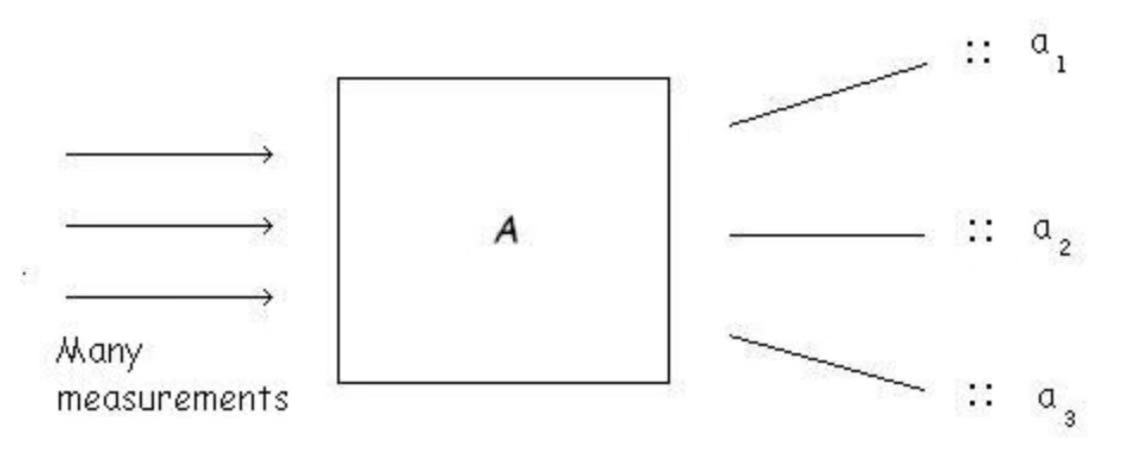
\includegraphics[width=8cm]{01.jpeg}
\end{figure}
\begin{IEEEeqnarray}{rLl}
P(a_1) = |C_{a_1}|^2 
\end{IEEEeqnarray}
\indent You measure only eigenvalues of $\hat{A}$.\\ 

More details about measurement can see CHEM356 Chapter\#4 notes.\\
\indent See Link: \href{http://scienide2.uwaterloo.ca/~nooijen/Chem356/Chem+356+pdf/Ch_4.pdf}{CHEM356 Chapter\#4 Notes} 


\section{Time-dependent Schr{\"o}dinger Equation}

 The fundamental starting point for non-relativistic quantum chemistry is the time-dependent Schr{\"o}dinger equation (T.D.S.E.):
\begin{IEEEeqnarray}{rLl}
i \hbar \frac{\partial \psi}{\partial t} = \hat{H} \psi \qquad \psi(t=0) = \psi_0  
\end{IEEEeqnarray}

\begin{itemize}
	\item $\psi_0$ is the initial condition to specify what is the wavefunction at time $t=0$. $\psi(r_1, r_2, ..., r_N, t)$ is a wavefunction that depends on all coordinates of the particles in the system and time. $\psi(r_1, r_2, ..., r_N, t)$ is extremely complicate. Even tabulation on a grid and solving as differential equation are impossible in quantum chemistry.
	\item $\hat{H}$ is an Hamiltonian operator for a system of electrons. The Hamiltonian operator is fairly simple to write down. It can be expressed as:
\begin{IEEEeqnarray}{rLl}
\hat{H} &= \hat{T} + \hat{V}  
\end{IEEEeqnarray}
\begin{itemize}
	\item[a)] $\hat{T}$ is the Kinetic energy.
\begin{IEEEeqnarray}{rLl}
\hat{T} &= -\hbar^2 \sum_{\alpha} \frac{1}{2m_{\alpha}} \nabla_{\alpha}^2 = \sum_{\alpha} \frac{p_{\alpha}^2}{2m_{\alpha}} \qquad  \\
\nabla_{\alpha}^2 &= (\frac{\partial^2}{\partial x^2} + \frac{\partial^2}{\partial y^2} + \frac{\partial^2}{\partial z^2})_{\alpha}     
\end{IEEEeqnarray}
	\item[b)]$\hat{V}$ is the Coulomb interaction. 
\begin{IEEEeqnarray}{rLl}
\hat{V} &= \sum_{\alpha \neq \beta} \frac{1}{4 \pi \epsilon_0} \frac{q_{\alpha}q_{\beta}}{|r_{\alpha}-r_{\beta} |} 
\end{IEEEeqnarray}	
	Here $q_{\alpha}$ is charge of particle $\alpha$, $r_{\alpha}$ is the position of particle $\alpha$.
\end{itemize}
	\item Assume no magnetic effects in the system.
	\item Assume no relativistic effects in the system.
	\item Assume no external fields in the system. If we add electric field in the system, we need consider $\sum_{\alpha} \mu_{\alpha} E_{\alpha}(r,t) $, where $\mu_{\alpha}$ is the dipole moment, and $E_{\alpha}(r,t)$ is the electric field of laser.
	\item This equation leaves out spin. We will introduce this later.
\end{itemize}

By integrating the T.D.S.E, we can calculate $|\psi(t) \rangle$ for all time, providing the wavefunction at $t=0$ is known.


\subsection{Time-independent Schr{\"o}dinger Equation}
We often need formally simplified the solution to T.D.S.E. Hence, we can firstly deal with the time-independent Schr{\"o}dinger Equation to get $\psi(t=0)$. For the time-independent Hamiltonian, the Schr{\"o}dinger equation:
\begin{IEEEeqnarray}{rLl} 
\hat{H} \phi_{n} &= E_n \phi_n  \\
\hat{H} |\phi_{n} \rangle &= E_n |\phi_n\rangle 
\end{IEEEeqnarray}	
\indent \qquad NOTE: $E_n$ is the energy of the eigenvalue.

We can express the wavefunction at $t=0$, using linear combinations of arbitrary $C_n$ and $\phi_n$.
\begin{IEEEeqnarray}{rLl} 
|\psi(t=0)\rangle &= \sum_{n} C_n |\phi_n\rangle \notag \\
\sum_{n} |C_n|^2 &= 1 \notag
\end{IEEEeqnarray}

\subsection{The Formal Solution to Time-dependent Schr{\"o}dinger Equation}
The solution of the time-dependent Schr{\"o}dinger equation is the wavefunction 
 $|\psi(t) \rangle$ for all time with the initial condition, $\psi_0$.\\
\indent As before, it is easy to verity that:
\begin{IEEEeqnarray}{rLl} 
i\hbar |\frac{\partial \psi}{\partial t}\rangle &= \hat{H}|\psi\rangle  \\
\hat{H}| \phi_n \rangle &= E_n | \phi_n \rangle  \\
| \psi_0\rangle &= \sum_n C_n | \phi_n \rangle 
\end{IEEEeqnarray}
\indent Hence, we can get $\psi(t)$ for all time.
\begin{IEEEeqnarray}{rLl} 
|\psi(t)\rangle &= \sum_{n} C_n e^{-iE_nt/ \hbar}|\phi_n\rangle  
\end{IEEEeqnarray}

\begin{itemize}
	\item Get coefficients $C_n(t)$ from phase factor, $e^{-iE_nt/ \hbar}$. Also, this is all time-dependent in Q.M.
	\item Conceptually, this is much simpler than classic mechanics.
\end{itemize}

\subsection{The Probability of Energy in Quantum Measurement}
The probability to find the energy, $E_m$, upon quantum measurement:
\begin{IEEEeqnarray}{rLl} 
C_m(t) &= C_m(0)e^{-iE_mt/ \hbar}  \\
P(E_m) &= C_m(t) C_m^*(t)  \\
&= C_m(0)e^{-iE_mt/ \hbar} C_m(0)e^{iE_mt/ \hbar}  \\
P(E_m,t) &= |C_m(0)|^2 =P(E_m,t=0) 
\end{IEEEeqnarray}
\indent According to the derivation, the excited states do not decay. However, this is not true in the real experiment. \\
\indent How to get the finite lifetime? \\
\indent Firstly, consider the quantum electronic dynamics. Treat electromagnetic radiation also at the quantum level (quantum ``photons"). Then, we can get the finite lifetime.\\
\indent \fbox{Very Complicated!}

Conclusion:\qquad \fbox{Wrong physics but useful!} \\
\indent \qquad Excited states do not decay.\\
\indent \qquad Excited states do not not reach equilibrium. The concept of temperature is not in Quantum \indent \qquad mechanics proper.\\
\indent \qquad $\Rightarrow \text{No thermal ensemble. The quantum mechanics cannot give Boltzmann distribution}$.\\
\indent \qquad Statmech is a layer on the top of quantum mechanics.

\paragraph{Boltzmann Distribution}~{}\\
\indent The eigenstate of the Hamiltonian $\hat{H}$ plays a concise role. It can create the thermal ensemble with energy. Properties are determined from a Boltzmann distribution.
\begin{IEEEeqnarray}{rLl} 
P_n &\sim e^{-E_n/K_BT}  \\
\langle \hat{O} \rangle &= \sum_n P_n \langle \psi_n|\hat{O}|\psi_n \rangle  
\end{IEEEeqnarray}
\indent \qquad Here $T$ is the temperature. Also, $|\psi_n\rangle$ denotes the complete set of eigenstates.
  
\subsection{Hamiltonian (Non-relativistic) for Quantum Chemistry}
\paragraph{Brief Introduction of Relativistic Quantum Mechanics}~\\
\indent We neglect magnetic/ spin-orbital effects in most of quantum chemistry, but there are ways to include major effects from relativity using so-called scalar contribution to relativity.\\
\indent The speed of electrons close to nuclei is a sizeable fraction of c, speed of light. When the velocity closed to 10\% of the speed of light, the relativistic effects start to become important. The relativity is important from $1^{st }$ transition metal. (This is done most easily and cleanly in the context of relativistic quantum mechanics.)
\begin{itemize}
\item If you have an external magnetic field or interactions of electrons, we usually need to consider the magnetic effects in Sch\"{o}dinger equation. This system is relativistic quantum mechanics. The key result is the Dirac equation, from which these prediction emerge automatically. By contrast, in non-relativistic quantum mechanics, terms have to be introduced artificially into Hamiltonian operator to achieve agreement with experimental observation.\\
\indent There are three effects naturally.
 \begin{itemize}
	\item[a)] Electron spin.
	\item[b)] Spin -orbital coupling.
	\item[c)] Magnetic field.(because spin is included naturally.)
\end{itemize}
\end{itemize}

\paragraph{Hamiltonian in Non-relativistic Quantum Chemistry}~\\
\indent Classical expression for energy of charged particles, neglecting magnetic effects:
\begin{IEEEeqnarray}{rLl} 
E =\sum_{\alpha} \frac{p_{\alpha}^2}{2m_{\alpha}} + \frac{1}{2}\sum_{\alpha \neq \beta} \frac{q_{\alpha}q_{\beta}}{4\pi\epsilon_0 |\textbf{r}_{\alpha}-\textbf{r}_{\beta}|}  
\end{IEEEeqnarray}
\begin{itemize}
	\item[-] Only electrostatic interaction
	\item[-] No Lorentz force/ magnetism. 
\end{itemize}
\indent \qquad The Hamiltonian in quantum mechanics:
\begin{IEEEeqnarray}{rLl} 
\hat{H}=\sum_{\alpha}-\frac{\hbar^2 \nabla_{\alpha}^2}{2m_{\alpha}}+\frac{1}{2}\sum_{\alpha \neq \beta}\frac{q_{\alpha}q_{\beta}}{4\pi\epsilon_0 |\textbf{r}_{\alpha}-\textbf{r}_{\beta}|}    
\end{IEEEeqnarray}
\begin{itemize}
	\item The expression of Kinetic energy is $\sum_{\alpha}-\frac{\hbar^2 \nabla_{\alpha}^2}{2m_{\alpha}}$.
	\item The expression of Coulomb energy is $\frac{1}{2}\sum_{\alpha \neq \beta}\frac{q_{\alpha}q_{\beta}}{4\pi\epsilon_0 |\textbf{r}_{\alpha}-\textbf{r}_{\beta}|}$.
	\item The expression of Nabla-squared $\nabla_{\alpha}^2$ is abuse of notation in Kinetic energy.
\begin{IEEEeqnarray}{rLl} 
&\hat{p}_x &= -i\hbar \frac{\partial}{\partial x}  \\
&\frac {\hat{p}_x^2}{2m} &= \frac{-\hbar^2}{2m} \frac{\partial^2}{\partial x^2}  \\
&\hat{T} &= \frac{p\cdot p}{2m} = -\frac{\hbar^2}{2m} \nabla\cdot\nabla  \\
&\nabla_{\alpha} &= (\frac{\partial}{\partial x} +\frac{\partial}{\partial y} + \frac{\partial}{\partial y})_{\alpha}  \\
&\nabla^2_{\alpha} &= (\frac{\partial^2}{\partial x^2} +\frac{\partial^2}{\partial y^2} + \frac{\partial^2}{\partial z^2})_{\alpha} 
 \end{IEEEeqnarray}
 \item Use atomic units (a.u.): $\hbar =m_e = e = a_o =1$, where $\hbar$ is reduced Planck constant, $e$ is elementary charge, $a_0$ is Bohr radius, and $m_e$ is electron mass. (Note: $4\pi\epsilon_0 =1$ in a.u.)\\
 \indent \qquad Why use atomic units?
 \begin{itemize} 
 \item[1)] Equations are simpler because we don't write any constants. \\
\indent \qquad e.g. Use the phase factor $\phi_n e^{-iE_nt}$ to instead of $\phi_n e^{-iE_nt/\hbar}$
  \item[2)]If you have the exact/accurate result in a.u., it will never change in calculations. In physical constants, $\hbar = \frac{h}{2\pi}= 1.054...\times 10^{-34} J\cdot s$. The value of $\hbar$ can change over time due to more precise measurements. Results never change when expressed in a.u.
\end{itemize}
\item The symbol,$\sum_{\alpha}$, inKinetic energy includes all particles, nuclei and electrons in the system. 
\end{itemize}




\indent The Schr\"{o}dinger equation with neglecting spin momentum can be expressed as:
\begin{IEEEeqnarray}{rLl} 
 \hat{H}\phi_n(r_1, r_2,...,r_n,R_1,R_2,...,R_Z) = E_n\phi_n 
 \end{IEEEeqnarray}
\indent \qquad \qquad \qquad \qquad $r_i$: electronic coordinate.
\indent \qquad $R_{\alpha}$: nuclear coordinate.\\
\indent \qquad \qquad \qquad \qquad $i$ labels as electrons, $\alpha$ labels as nuclei.\\

\indent Direct Solution of this problem is very complicated. The solution separates off overall translation (particle in the box in Q.M.), but still includes rotational, vibrational, and electronic degrees of freedom.\\
\indent It has been done for very small molecules. e.g. LiH, BH, etc. (Center of mass is taken out)\\
\indent In practice one proceeds in steps.
\begin{IEEEeqnarray}{rLl} 
 \hat{H} &= \underbrace{ \sum_{\alpha}-\frac{1}{2}\frac{\nabla_{\alpha}^2}{M_\alpha}}_{\text{kinetic energy of nuclei}}+\underbrace{ \sum_i -\frac{1}{2}\nabla_i^2}_{\text{kinetic energy of electrons}}+\underbrace{ \frac{1}{2}\sum_{\alpha\neq\beta}\frac{Z_\alpha Z_\beta}{R_{\alpha\beta}}}_{\text{nuclear repulsion}}+\underbrace{\sum_{\alpha,i}-\frac{Z_\alpha}{r_{\alpha i}}}_{\text{Coulomb energy of $\alpha$ \& i}} +\underbrace{ \frac{1}{2}\sum_{i\neq j}\frac{1}{r_{ij}}}_{\text{Coulomb energy between electrons}}  \\
  &= \hat{T}_N + \hat{T}_{ele} + \hat{V}_{NN} + \hat{V}_{Ne} +\hat{V}_{ele} 
  \end{IEEEeqnarray}
\indent NOTE: Disregard the kinetic energy of nuclei, $\hat{T}_N$. This term is treated separately later.



\subsection{Clamped Nuclei}
\begin{itemize}
\item [Step 1:]  Fix the molecular geometry, $\vec{R_{\alpha}}$ \qquad $\vec{R_1}$, $\vec{R_2}$, ...,$\vec{R_N}$.\\
Assume fixed positions of nuclei. Solve problems for the electrons for the particular nuclear geometry. (major task)\\
How to indicate the clamped nuclei?\\
We indicate clamped nuclei by the semi colon. e.g. $\psi_{\lambda}^{el}(\underbrace{\vec{r_1},\vec{r_2},...\vec{r_N}}_{\text{all electrons}};\underbrace{\vec{R_1},\vec{R_2},...,\vec{R_Z}}_{\text{all fixed nuclei}})$.\\

 Solve for the clamped nuclei solutions:
\begin{IEEEeqnarray}{rLl} 
\hat{H}_{el}\{\vec{R}\} \psi_{\lambda}^{el}(\{\vec{r}\};\{\vec{R}\}) = E_{\lambda}\{\vec{R}\}\psi_{\lambda}^{el}(\{\vec{r}\};\{\vec{R}\}) 
\end{IEEEeqnarray}
NOTE:\\
	The energy, $E_{\lambda}\{\vec{R}\}$, depends on nuclear coordinates due to the nuclear configuration. It means that if we change the nuclear position and solve for the Schr\"{o}dinger equation, we can get different points on the potential energy surface.\\
\hangindent 7em
\hangafter=0

\item [Step 2:]  The solution (wavefunction) to the full nuclear + electrons Schr\"{o}dinger equation can be written as: (in exact expansion)
\begin{IEEEeqnarray}{rLl} 
\phi_n (\{\vec{r}\},\{\vec{R}\})= \sum_{\lambda} \psi_{\lambda}^{el}(\{\vec{r}\};\{\vec{R}\}) \chi_{\lambda}	\{\vec{R}\}  
\end{IEEEeqnarray}
The electronic clamped nuclei states are used as an expression set (basis):
\begin{IEEEeqnarray}{rLl} 
(\hat{T}_N+\hat{H}_{el})\sum_{\lambda}\psi_{\lambda}^{el}(\{\vec{r}\};\{\vec{R}\})\chi_{\lambda}	\{\vec{R}\} = E \sum_{\lambda} \psi_{\lambda}^{el}(\{\vec{r}\};\{\vec{R}\})\chi_{\lambda}\{\vec{R}\}   
\end{IEEEeqnarray}
NOTE:\\
	The energy, $E$, is the constant. The second step is to calculate the full vibrational problem. This solution refers to vibronic coupling problem by coupling different electronic states. \\
\hangindent 7em
\hangafter=0
\end{itemize}

\section{Electronic Structure Problem}
Focus on electronic structure problem. Assume fixed positions of nuclei. Solve problems for the electrons for the particular fixed nuclear geometry. Solve for the Schr\"{o}dinger equation:
\begin{IEEEeqnarray}{rLl} 
\hat{H}_{el}\{\vec{R}\} \psi_{\lambda}^{el}(\{\vec{r}\};\{\vec{R}\}) = E_{\lambda}\{\vec{R}\}\psi_{\lambda}^{el}(\{\vec{r}\};\{\vec{R}\}) 
\end{IEEEeqnarray}
\indent From electronic structure, we can calculate potential energy curve under each different geometries for both ground state and excited states.
\begin{figure}[htp]
    \centering
    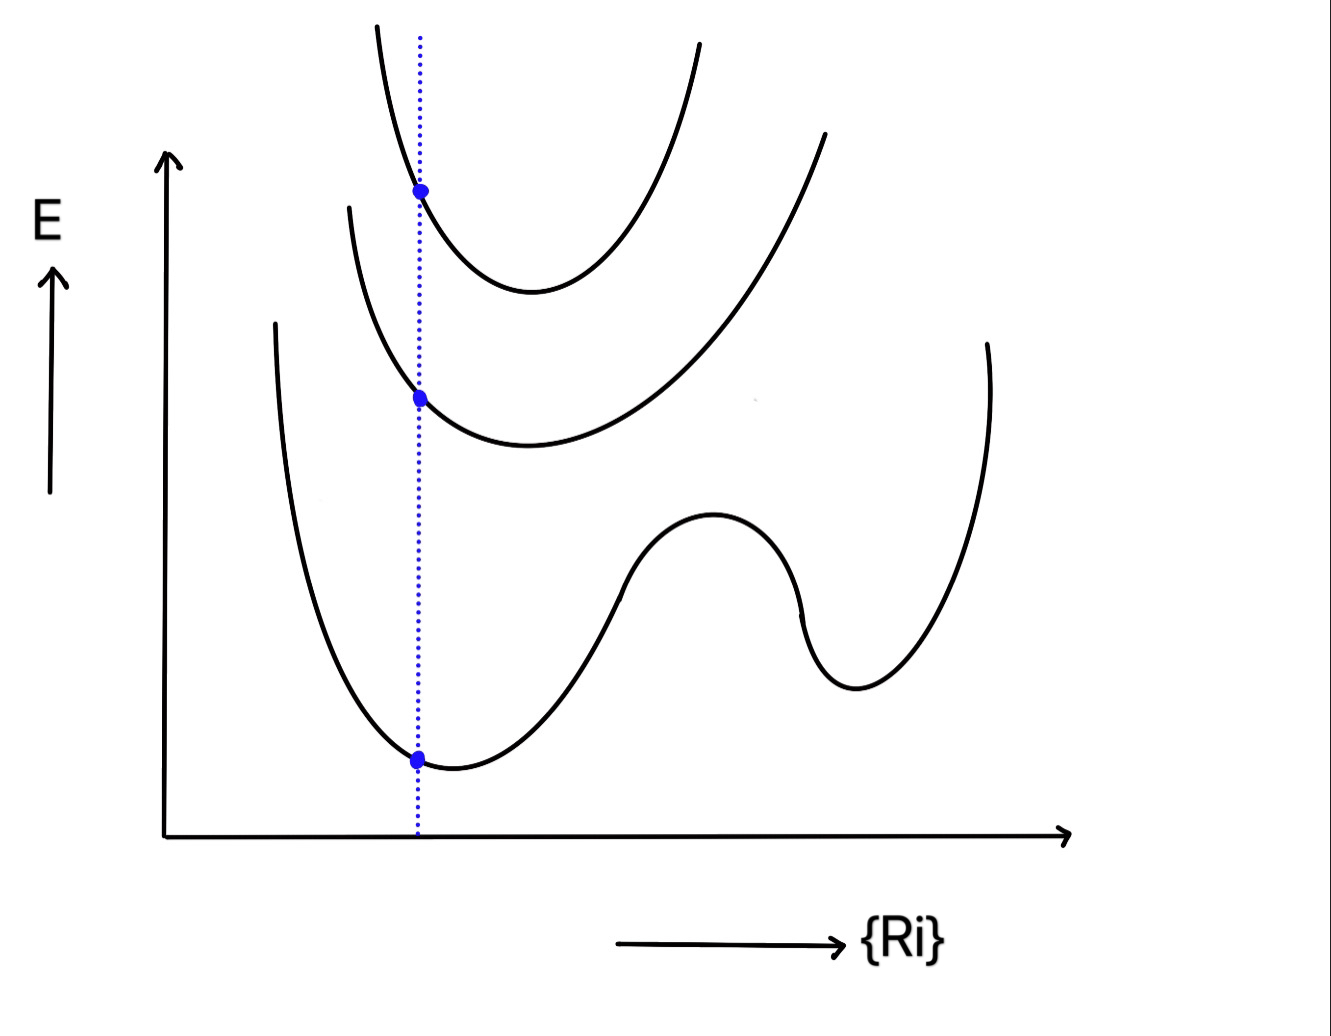
\includegraphics[width=6cm]{02.JPG}
\end{figure}

\subsection{Born-Oppenheimer Approximation}
Describe the wavefunctions within Born-Oppenheimer approximation by a single surface (electronic state). The nuclei move on a potential energy surface obtained by solving the electronic problem. Here is the solution, the full wavefunction:
\begin{IEEEeqnarray}{rLl} 
\phi_n (\{\vec{r}\},\{\vec{R}\})= \psi_{0}^{el}(\{\vec{r}\};\{\vec{R}\}) \cdot\chi_{n}\{\vec{R}\}  
\end{IEEEeqnarray}
\indent NOTE: There are different rovibrational levels $\phi_n$, $E_n$.\\
\indent This is not an exact solution, but very accurate. The groundstate is ``well separated" from electronic excited states, $\psi_{\lambda}(\{\vec{r}\};\{\vec{R}\})$, with $\lambda=1,2,3,...$.\\
\indent ``well separated" means the number of $E_{\lambda}-E_0$ is large for relevant geometry $\{R\}$.\\
\indent e.g. $E_{\lambda}-E_0 \gtrsim 3eV \approx 3\times800 = 32000 cm^{-1}$ \\
\indent $\Longrightarrow$ very large compared to rovibrational energy level.\\
\indent  This is the reason why the Born-Oppenheimer approximation works well. It assumes that nuclei are much heavier than electrons and they move more slowly. Hence, to a good approximation, the electrons in a molecule to be moving in the field or fixed nuclei.

I do not like stationary like: electrons move very fast compared to nuclei.\\
\indent $\Longrightarrow$ instantaneously adjust to position nuclei.\\
\indent The T.I.S.E. $\hat{H}\phi_n = E_n \phi_n$. What is moving? No motion for electrons.\\

\indent The Born-Oppenheimer approximation is not often suited for excited states because they are close in energy.\\
\indent $\Longrightarrow$ vibronic coupling = rovibrational-electronic coupling.\\
\indent $\Longrightarrow$ multiple electronic states are needed to describe nuclear motion.\\
\indent B.O approximation underlines chemistry molecular structure.

\subsection{Further Discussion of Quantum Chemistry in Practice}
Practical Goal:
\begin{itemize}
	\item Find stationary points on ground state potential energy surface.\\
\qquad The first minima of the potential energy at $\{R_1\}$ position.\\
\qquad The second minima of the potential energy at $\{R_2\}$ position.\\
	\begin{figure}[htp]
    \centering
    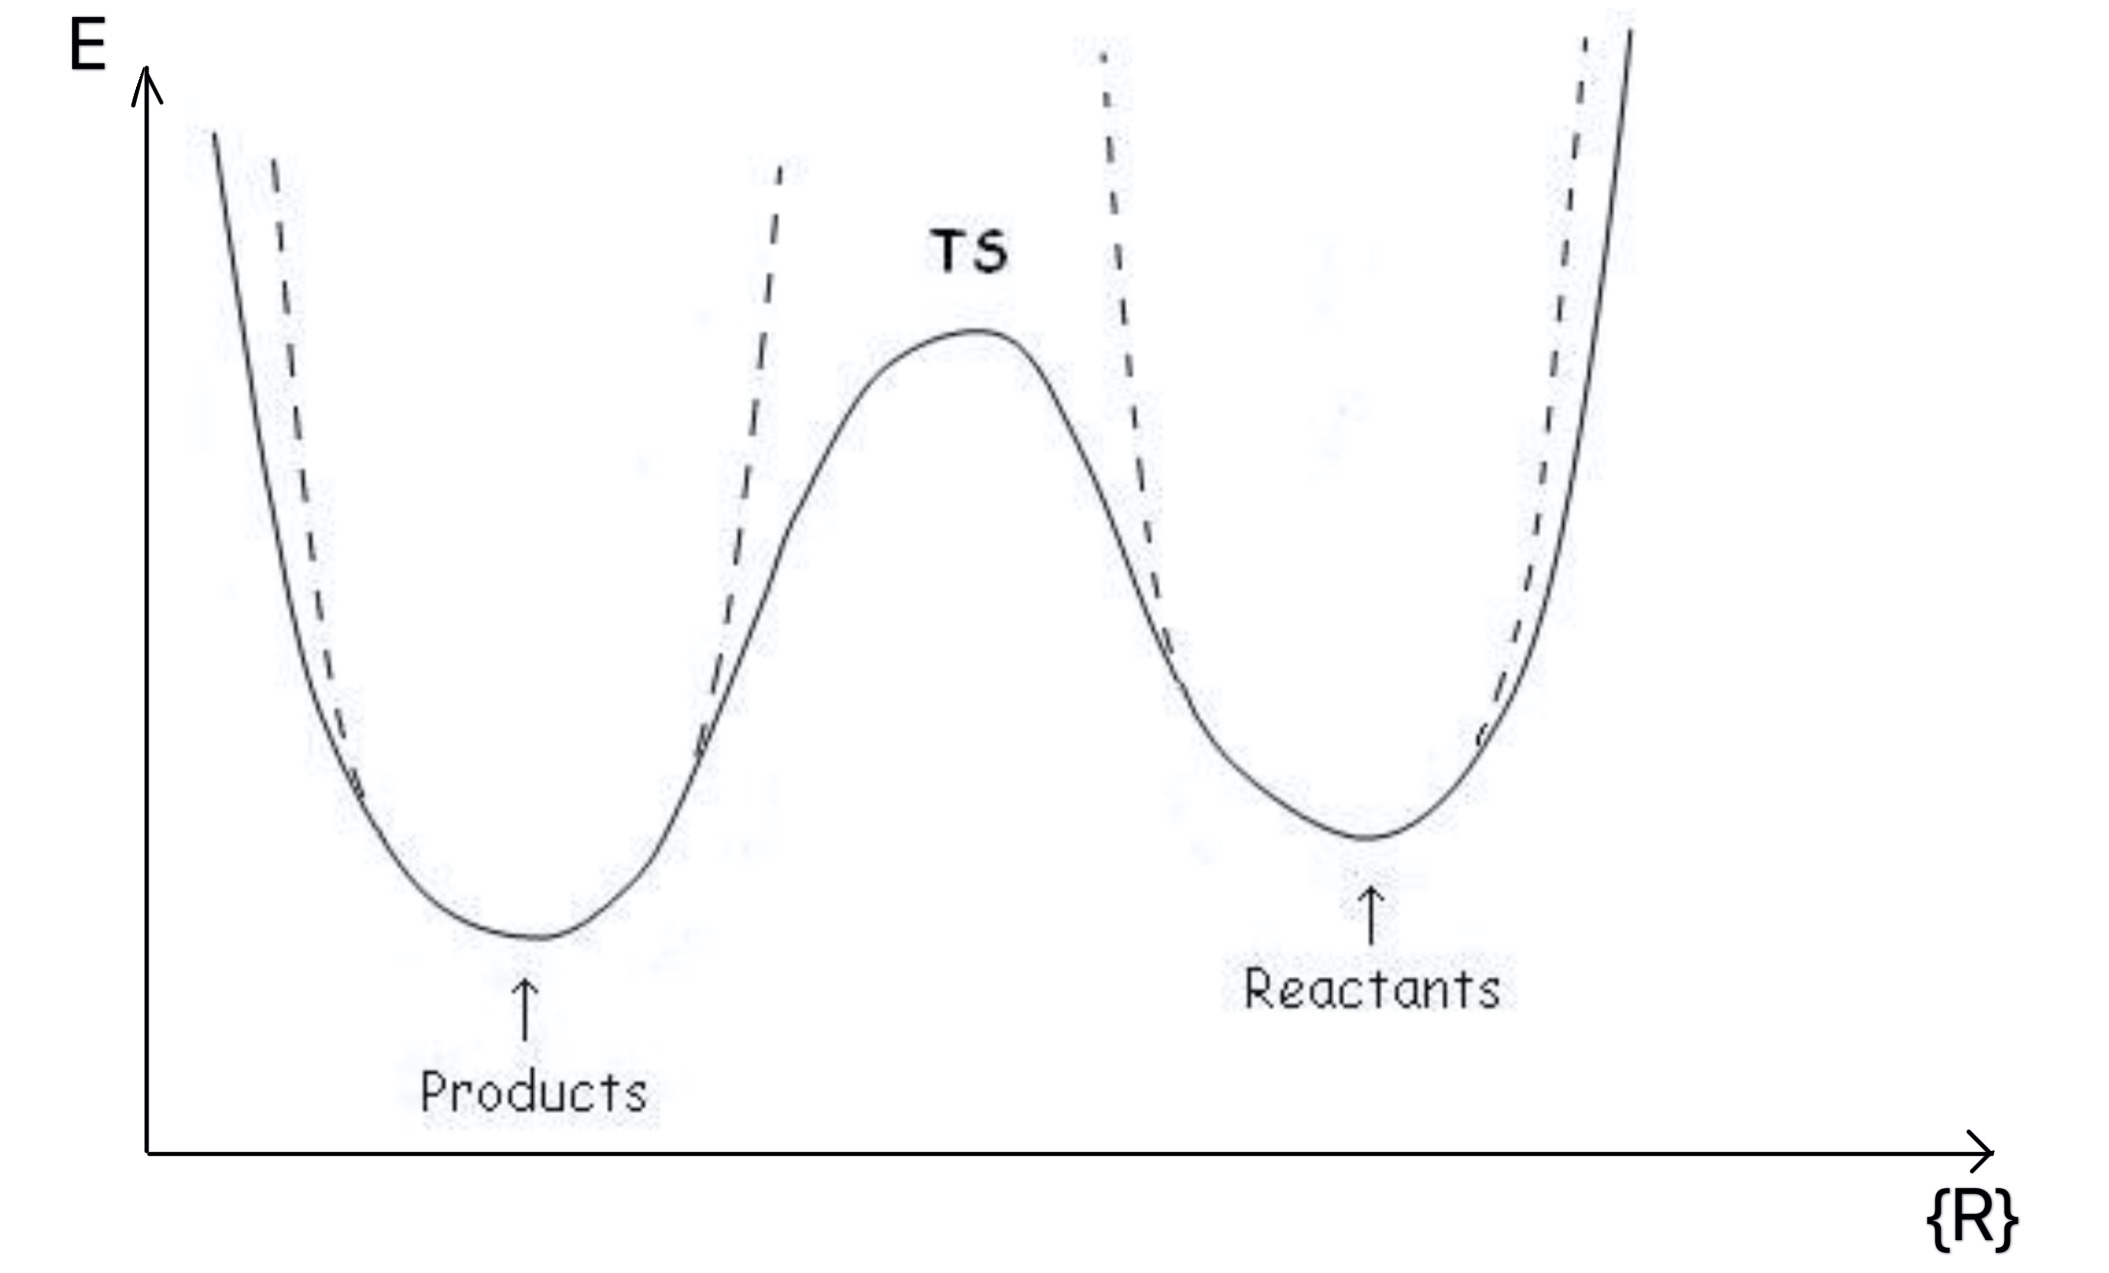
\includegraphics[width=8cm]{03.jpeg}
	\end{figure}
$\{R_1\}$ and $\{R_2\}$ represent stable molecular structures.\\
Transition state (TS): first order saddle points. Go up in all directions but one one (Reaction coordinates).
	\item Module to calculate: low lying local minima, $E_{\lambda}\{\vec{R}\}$.\\
$\Longrightarrow$ the position at minimum $\vec{R}_{min}$, \\
$\Longrightarrow$ the force constant matrix at minimum $K$\\
$\Longrightarrow$ the energy of ground state at minimum $E_{gs}(\vec{R}_{min})$
	\item Most common electronic structure (E.S.) calculations:\\
	Density Functional Theory (DFT) type $\Longrightarrow$ specify functional e.g. B3-Lyp.\\
	DFT is very good for geometries $\vec{R}_{min}$ and force constant matrix $K$.\\
	DFT is less good for energy at minimum $E_0\{\vec{R}_{min}\}$.\\
	$\Longrightarrow$ need more accurate method, like coupled cluster method.\\
	
	NOTE: DFT and coupled cluster are very different methods to approximate Schr\"{o}dinger Equation. Do Coupled Cluster calculation at converged DFT geometry.
	
	\item Here is the potential energy surface (PES) of the ground state energy, $E_0\{\vec{R}\}_{g.s}$.\\
	\begin{figure}[htp]
    \centering
    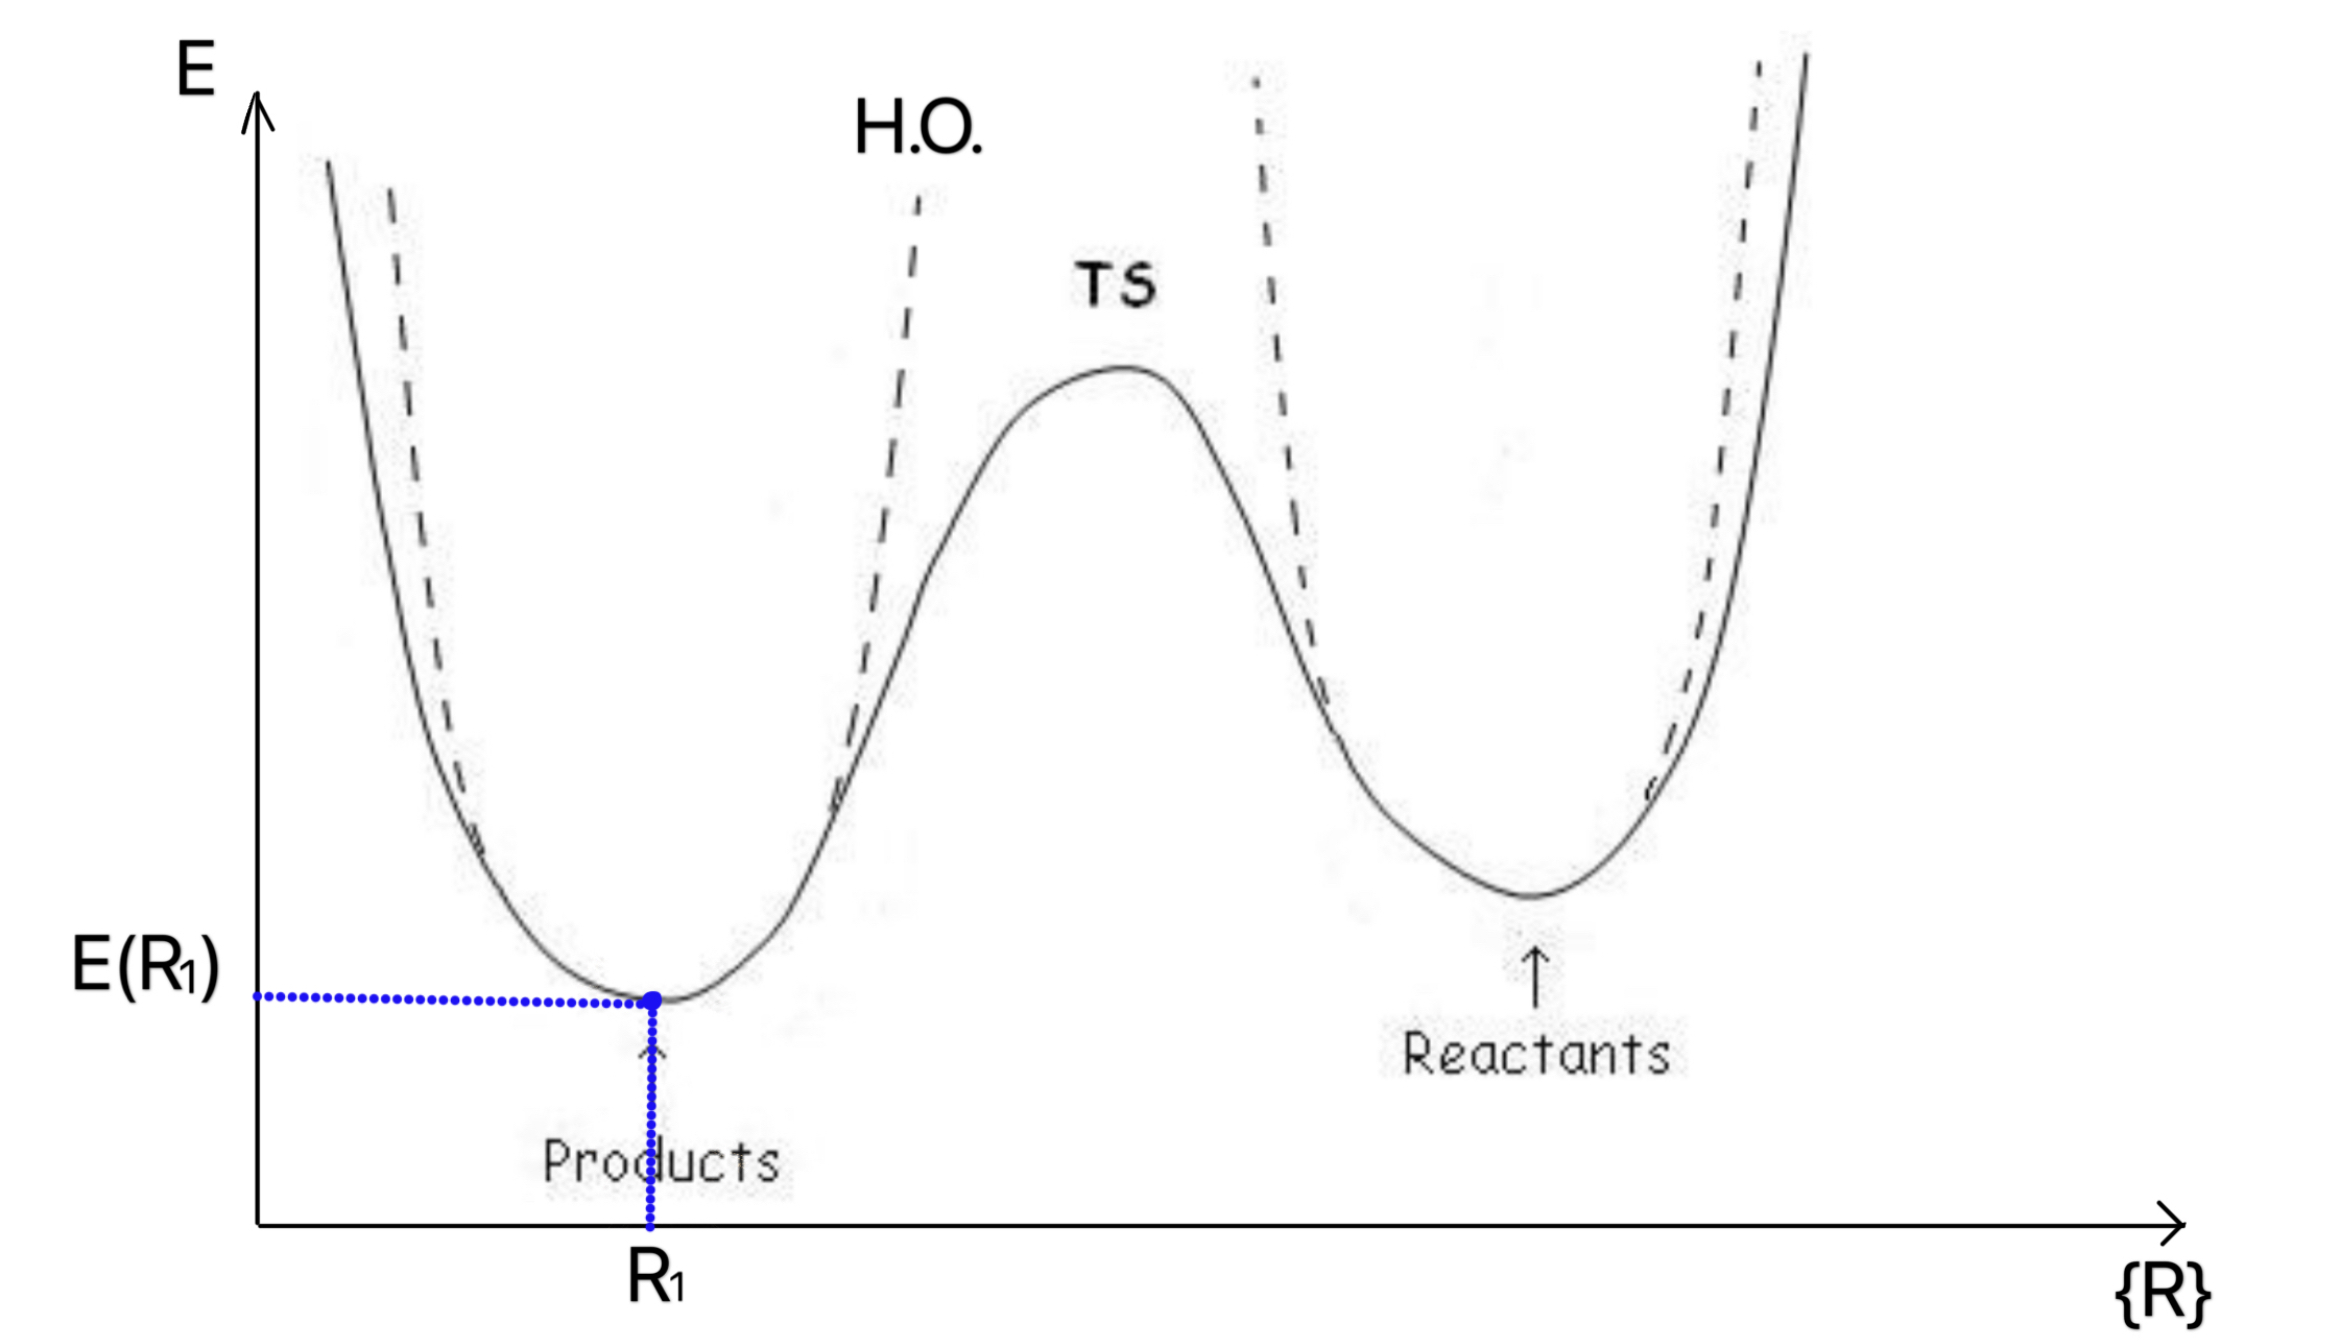
\includegraphics[width=8cm]{04.jpg}
	\end{figure}\\
	\begin{itemize}
	\item[1)] The potential energy surface by Harmonic Oscillator depends on the force constant matrix, $K$. The $K$ matrix is $3N \ast 3N$ matrix. \\
	$K_{\alpha i,\beta j}$, where $\alpha, \beta$ represent nuclei (N), and $i,j$ represent x,y,z Cartesian coordinates.
	\item[2)] For the Harmonic potential (quadratic potential), the gradient at minimum stationary point:
	\begin{IEEEeqnarray}{rLl} 
	 g_{\alpha,i} = \frac{\partial E}{\partial R_{\alpha,i}}=0 
	\end{IEEEeqnarray}
 NOTE: The Harmonic potential is also called Hessian, labeled as $K$ matrix for force constant.
 	\item[3)] Manipulations with masses, then diagonalize the $K_{\alpha i,\beta j}$ matrix to get $w_i^2$. The eigenvalue of the $K$ matrix is $w_i^2$, where $w_i$ represents vibrational frequencies.
 	\item[4)] A molecule with N atoms has 3N degrees of freedom.\\
 	- 3 overall translations.\\
 	- 3 overall rotations for non-linear molecule or 2 rotations for linear molecule.\\
 	- (3N-6) vibrations for non-linear molecule or (3N-5) vibrations for linear molecule.\\
 	
 	
	Example for non-linear molecule, $H_2O$:\\
	3 translations in water molecule. Electronic energy does not change under translation.\\
	3 eigenvalues with the number of 0, eigenvectors of the $K$ represent overall translations.\\
	3 rotations in water molecule. Electronic energy does not change under rotation.\\
	3 eigenvalues with the number of 0.\\
	
	In total, 6 eigenvalues with the number of 0, corresponding with translational / rotational motion. \\
	$w_i^2 \rightarrow w_i \rightarrow$ physically significant.\\
	At minimum: all $w_i^2$ values are positive, $w_i$ values are also positive.\\
	\begin{figure}[htp]
    \centering
    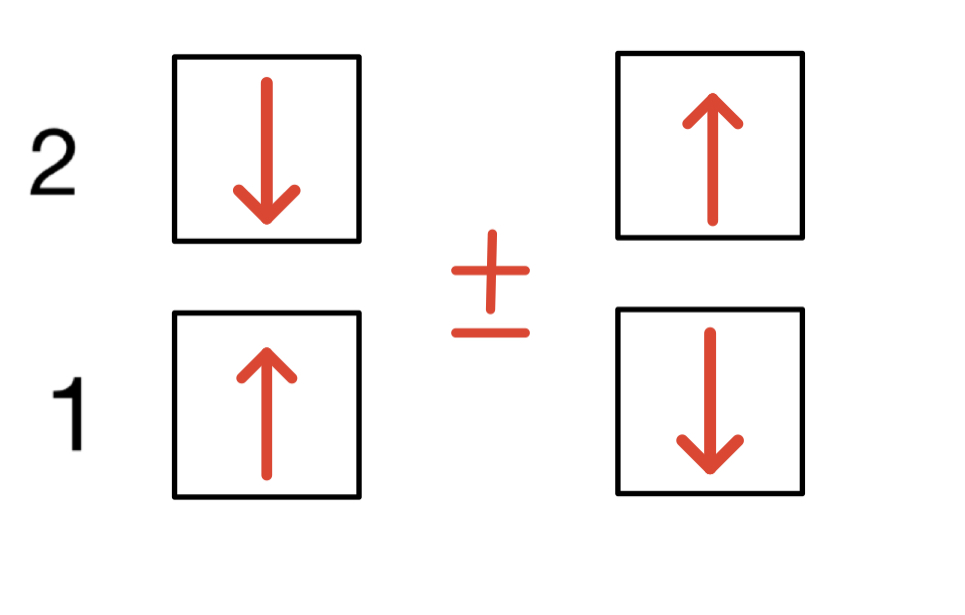
\includegraphics[width=6cm]{07.jpg}
	\end{figure}\\
	The difference between two adjacent energy levels: $\hbar \omega$.\\
	The zero point energy: $E_0 = \frac{1}{2}\hbar \omega$.\\
	\begin{figure}[htp]
    \centering
    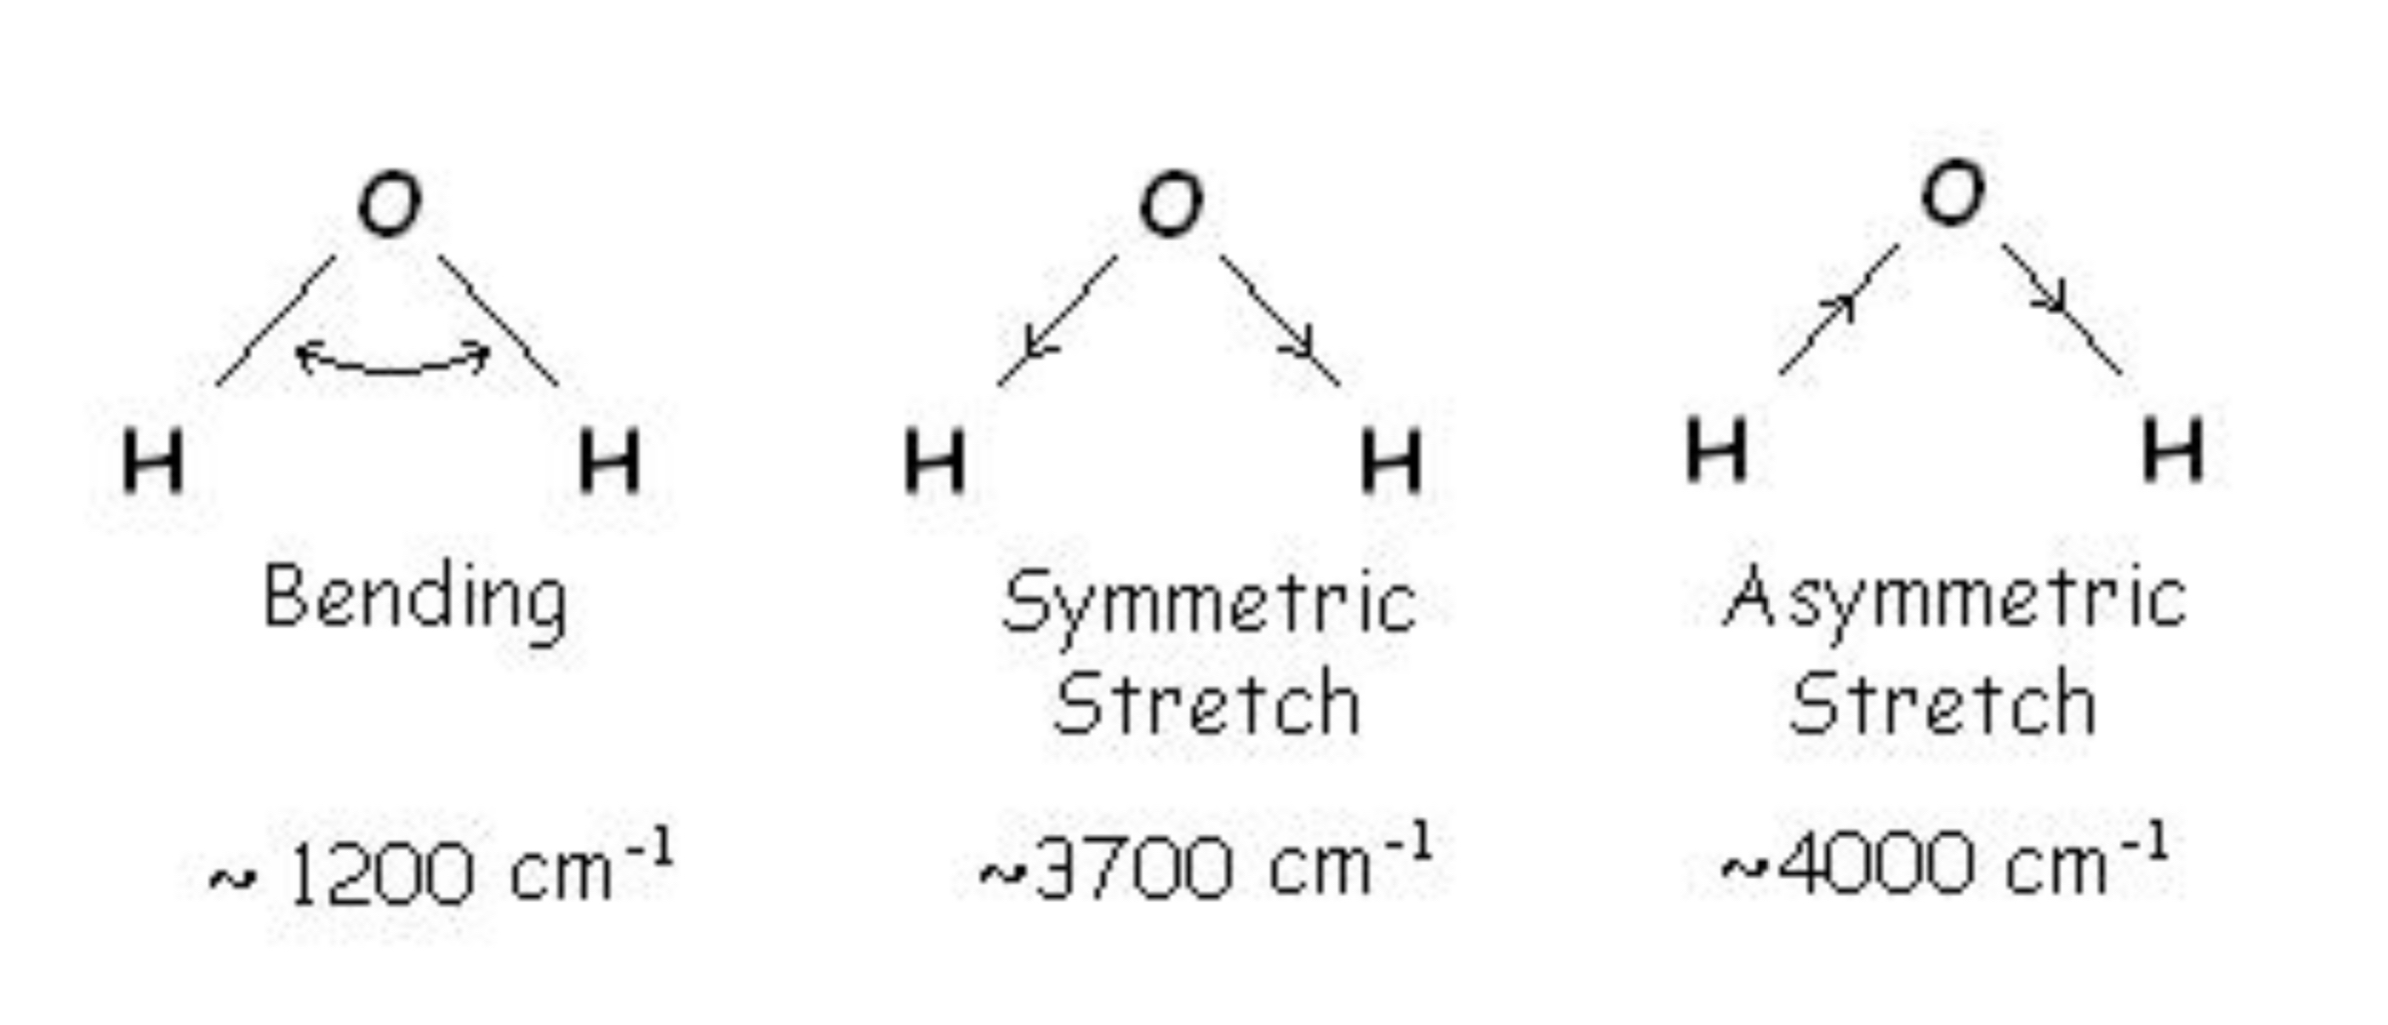
\includegraphics[width=12cm]{05.jpg}
	\end{figure}\\
	There are 3 different vibrational energies. e.g. 3N-6 = 3$\times$3 =3.\\
	Characterize vibrational states:
	\begin{IEEEeqnarray}{rLl} 
	&\text{vibrational states:} \qquad &|n_1, n_2, n_3 \rangle \notag \\
	&\text{ground state:} \qquad &|0, 0, 0 \rangle \qquad \frac{1}{2}\hbar\sum_{i}\omega_{i} =\frac{1}{2}(1200+3700+4000)=4400\text{cm}^{-1} \notag \\
	&\text{excited state:} \qquad &|1, 0, 0 \rangle \qquad \text{bending: 1200cm}^{-1} \notag 	\\
	&\text{excited state:} \qquad &|0, 1, 0 \rangle \qquad \text{symmetric stretch: 3700cm}^{-1} \notag \\
	&\text{excited state:} \qquad &|2, 1, 0 \rangle \qquad 2\times1200+1\times3700+0+E_{g.s.} \notag 
	\end{IEEEeqnarray}
	NOTE: All info on vibrational levels from Hessian or force constant matrix, $K$.\\
	$\Longrightarrow$ easily do sums: $\sum_{v=0,1,...}e^{-\beta E_{\text{vibrations}}}$(CHEM350: stat mech).\\
		
		
	Example for linear molecule, $CO_2$:\\
	3 translational modes for carbon dioxide molecule.\\
	2 rotational degrees of freedom  for carbon dioxide molecule. \\
	In total, there are (3N-5) vibrational frequencies for linear molecule. For carbon dioxide, there are 4 vibrational modes. \\
	\begin{figure}[htp]
    \centering
    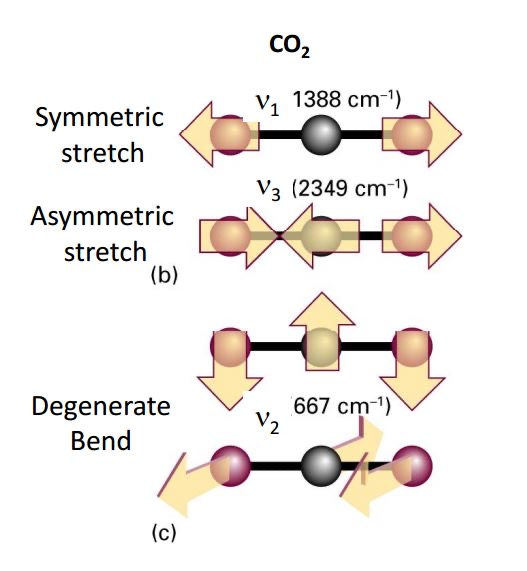
\includegraphics[width=8cm]{06.JPG}
	\end{figure}\\
	
	More details about Vibrational Modes:\\
	See Link: \href{http://scienide2.uwaterloo.ca/~nooijen/Chem356/Chem+356+pdf/Ch_5.pdf}{CHEM356 Chapter\#5 Notes} \\
	
	
	
	\item[5)] Rotational motions:\\
	There are rotational energy levels due to the nuclear motion. For diatomics and linear molecules we have simple formulas:
	\begin{IEEEeqnarray}{rLl} 
	E &= \frac{\hbar^2}{\mu R_e^2}J(J+1) = B_v J(J+1)     \\
	I_{\alpha\beta} &= \mu R^2 \\
	B_v &= \frac{\hbar^2}{\mu R_e^2}= \frac{\hbar^2}{2I} 
	\end{IEEEeqnarray}
	NOTE: $B_v$ is the rotational constant, and $ I_{\alpha\beta}$ is moment of inertia from Rigid Rotor quantum mechanics. For general polyatomic molecules the formulas are more complicated, but rigid rotor ure rotations are easily calculated on a computer. We mostly need only high temperature limit for Statmech thermal corrections.
	
	Here is the rotational spectrum for Harmonic Oscillator + Rigid Rotator:
	\begin{figure}[htp]
    \centering
    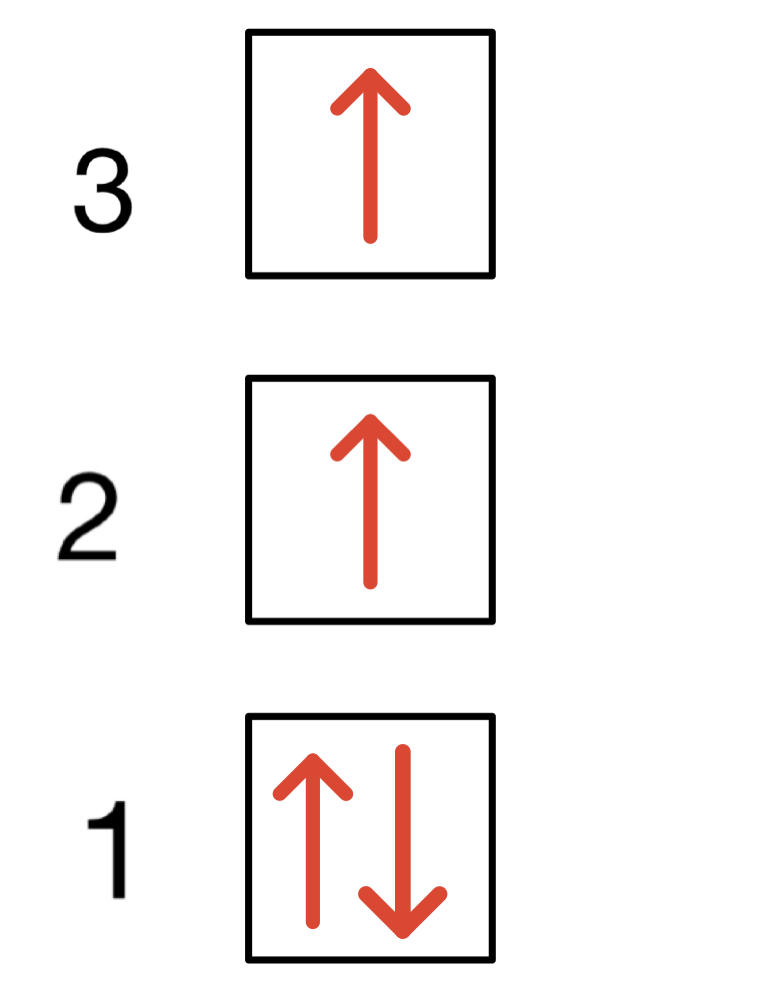
\includegraphics[width=10cm]{08.jpg}
	\end{figure}\\
		
	More details about Rotational Modes:\\
	See Link: \href{http://scienide2.uwaterloo.ca/~nooijen/Chem356/Chem+356+pdf/Ch_6.pdf}{CHEM356 Chapter\#6 Notes} \\
	More details about Thermal Corrections:\\
	See Link: \href{http://scienide2.uwaterloo.ca/~nooijen/website_new_20_10_2011/Chem350_statmech/Ch_5_statmech_chemistry.pdf}{CHEM350: Statistical Mechanics} \\
		
	\item[6)] To describe rotations, we need nuclear geometry, $R_{\alpha,i}$, to get moment of inertia, $I_{ij}$, where $i,j$ run over x,y,z Cartesian coordinates. \\
	The moment of inertia, $I_{ij}$, is 3$\times$3 matrix, and can get 3 eigenvalues for rotational motion.

	\end{itemize}
	
\end{itemize}

\begin{summary}{}{}
   If we can calculate:
    \begin{itemize}
    	\item  $\vec{R}_{\alpha,i}$: position of nuclei at stationary point, $\alpha=1,2,...,N$, i = x,y,z cartesian coordinates.
    	\item $K_{\alpha i,\beta j}$: force constant matrix.
    	\item $E(\vec{R}_{\alpha, i})$: energy at minimum.
    	\item $I_{\alpha,\beta}(\vec{R})$: moment of inertia.
    \end{itemize}
    
    \indent We can calculate the thermochemistry with good degree of accuracy, such as: equilibrium constants including transition state, rates of reactions.\\
     \indent Electronic structure problem is the central problem.   
\end{summary}

More details here:
    \begin{itemize}
    \item Calculate $E(\vec{R}_{\alpha})$, where $R_{\alpha}$ represents 3N coordinates to instead of $R_{\alpha,i}$.
    \item Calculate the gradient,
	\begin{IEEEeqnarray}{rLl} 
	 g_{\alpha,i} &= \frac{\partial E}{\partial R_{\alpha,i}}\Longrightarrow \text{cheap enough}  \\
	 K_{\alpha \beta} &=  \frac{\partial^2 E}{\partial R_{\alpha}\partial R_{\beta}} \Longrightarrow \text{Hessian, expensive} 
	\end{IEEEeqnarray}
	\item Optimize the geometry by finding minima where $g_\alpha = 0$.
	\item Make a potential energy surface with $E(R_i)$, $g(R_i)$, $K(R_i)$.
	\begin{IEEEeqnarray}{rLl} 
	E(x)=E(R)+\sum_i g_i x_i +\frac{1}{2}\sum_{i,j}x_iK_{ij}x_j
	\end{IEEEeqnarray}

NOTE: \\
\tab $\vec{x}$ is the displacement from $\vec{R_i}$.
	\begin{IEEEeqnarray}{rLl} 
	E(x) &=E_0+\sum_i g_i x_i +\frac{1}{2}\sum_{i,j}x_iK_{ij}x_j  \\
	\frac{\partial E}{\partial x_k} &=0 
	\end{IEEEeqnarray}
NOTE: \\
\tab $k$ is different from $i,j$.\\
\tab $E_0, g_i, K_{ij}$ are constants. \\
\tab $x_i$:  $x_1, x_2,...,x_{3N}$ independant coordinates.
	\begin{IEEEeqnarray}{rLl} 
	\frac{\partial x_i}{\partial x_k} =\delta_{ik}= \left\{
\begin{aligned}
	 1 \qquad \text{iff  i = k} ,\\
	 0 \qquad \text{iff  i $\neq$ k} .
\end{aligned}
\right. 
\end{IEEEeqnarray}



	\begin{IEEEeqnarray}{rLl} 
&\Longrightarrow 	\frac{\partial E}{\partial x_k} = 0+ \sum_i g_i \delta_{ik}+\frac{1}{2}\sum_{i,j} \delta_{ik}k_{ij}x_j+\frac{1}{2}\sum_{i,j} x_ik_{ij}\delta_{jk}	\\
&\Longrightarrow 	\frac{\partial E}{\partial x_k} = 	g_k + \underbrace{\frac{1}{2}\sum_{i,j} K_{kj}x_j+\frac{1}{2}\sum_{i,j} x_i K_{ij}}_{K_{kj}=K_{jk} \quad \text{ symmetric}}   \\
&\Longrightarrow  g_k + \sum_j K_{kj}x_j =0 \quad \text{(linear equation for }x_j) 
\end{IEEEeqnarray}

    	
    \end{itemize}

\subsection{General Solution to Electronic Schr\"{o}dinger Equation}
Rewrite electronic Schr\"{o}dinger equation: 
\begin{IEEEeqnarray}{rLl} 
\hat{H}^{el}(\{\vec{R}\}) \psi_{\lambda}^{el}(\vec{r},\vec{R}) = E_{\lambda}(\vec{R})\psi_{\lambda}^{el}(\vec{r},\vec{R})
\end{IEEEeqnarray}
\tab From now on we will suppress the $\vec{R}$ displacement, and drop the subscript $`el'$, then: 
\begin{IEEEeqnarray}{rLl} 
\hat{H} \psi(\vec{r}) &= E \psi(\vec{r})  \\
\hat{H} &= \hat{T}_e + V^{Ne} + V^{ee} \notag \\
&= \sum_i -\frac{1}{2} 	\nabla_i^2 +\sum_{\alpha,i} -\frac{Z_{\alpha}}{|r_i-R_{\alpha}|} + \frac{1}{2} \sum_{i<j} \frac{1}{r_{ij}}	 \\
&= \sum_i (-\frac{1}{2}\nabla_i^2 +V(r_i)) + \frac{1}{2} \sum_{i<j} \frac{1}{r_{ij}} \\
&\equiv \sum_i h(i) + \frac{1}{2}\sum_{i \neq j} \frac{1}{r_{ij}}  \\
&\equiv \hat{h} + \hat{V}  
\end{IEEEeqnarray}

NOTE: \\
\tab\tab  $\vec{r}$: electron coordinates.\\
\tab\tab $\hat{h}$ is one-electron operator.\\
\tab \tab $\hat{V}$ is two-electron operator. \\
\tab \tab $V_{NN}$ is just a constant which can be added to energy.(important when calculate PES) \\

\subsubsection{One-electron Hamiltonian}
To understand the structure of solution let us firstly consider the one-body Hamiltonian.
\begin{IEEEeqnarray}{rLl} 
\hat{H} = \sum_i \hat{h}(i)  
\end{IEEEeqnarray}
\tab We can solve the S.E. for this problem by postulating that the wave function in a product of one-electron functions (orbitals).
\begin{IEEEeqnarray}{rLl} 
\psi(1,2,...,N) = \psi_a(1) \psi_b(2) \cdots \psi_Z(N)  
\end{IEEEeqnarray}
\tab Then:
\begin{IEEEeqnarray}{rLl} 
&(\hat{h}(1)+\hat{h}(2)+\cdots +\hat{h}(N) )(\psi_a(1) \psi_b(2) \cdots \psi_Z(N))  \notag\\
& = (\hat{h}(1)\psi_a(1))  \psi_b(2) \cdots \psi_Z(N) \notag \\
&+(\hat{h}(2)\psi_b(2)) \psi_a(1) \cdots \psi_Z(N) \notag \\
&+ \cdots \notag \\
&+ (\hat{h}(N)\psi_Z(N)) \psi_a(1)  \cdots \psi_Z(N) 
\end{IEEEeqnarray}
\tab NOTE:\\
\tab \tab Why?\qquad $\hat{h}(1)=-\frac{1}{2} 	\nabla_1^2 + V(1)$\\
\tab \tab The derivative acts only on $\psi_a(1)$. Multiplication is done once, etc.\\

Therefore, the equation is divided by $\psi$.
\begin{IEEEeqnarray}{rLl} 
\frac{\hat{h}(1)\psi_a(1)}{\psi_a(1)} + \frac{\hat{h}(2)\psi_b(2)}{\psi_b(2)} + \cdots + \frac{\hat{h}(N)\psi_Z(N)}{\psi_Z(N)} = \frac{E\psi}{\psi} = E \notag
\end{IEEEeqnarray}

Following standard reasoning in separation of variable, each term has to be a constant.
\begin{IEEEeqnarray}{rLl} 
&\hat{h}(1)\psi_a(1)&= \varepsilon_a \psi_a(1)  \\
&\hat{h}(2)\psi_b(2)&= \varepsilon_b \psi_b(2)  \\
&\vdots &\vdots \notag \\
&\hat{h}(N)\psi_Z(N)&= \varepsilon_Z \psi_Z(N)  \\
&E = \varepsilon_a + \varepsilon_b &+ \cdots + \varepsilon_Z 
\end{IEEEeqnarray}

Moreover every $\hat{h}(i)$ is the same operator, only coordinate is named differently. \\
\tab $\Longrightarrow$ Solve one electron problem to get many solutions $\varepsilon, \psi_a(1)$ (eigenvalues, eigenfunctions).
\begin{IEEEeqnarray}{rLl} 
\hat{h}(1)\psi_a(1) = \varepsilon_a \psi_a(1)  
\end{IEEEeqnarray}
\tab NOTE:\\
\tab\tab $\varepsilon_a$: orbital energies.\\ 
\tab\tab $\psi_a(1)$: orbitals: one-electron eigenfunctions of $\hat{h}(1)$.\\


\subsubsection{Many-electron Hamiltonian}
Once I have solved the one-electron problem, one can write solutions for many-electron wave functions. 
\begin{IEEEeqnarray}{rLl} 
\psi_{\lambda} &= \psi_a(1)\psi_b(2)\cdots\psi_Z(N)  \\
E_{\lambda} &= \varepsilon_a +\varepsilon_b +\cdots + \varepsilon_Z 
\end{IEEEeqnarray}

Pick N orbitals, $\psi_a, \psi_b,..., \psi_Z$\\
\tab $\Longrightarrow \psi, E$, $E$ is the sum of orbital energies.

Question: What is the ground state of this Hamiltonian $\hat{h}$?\\
\indent Answer: Put all electrons in the lowest energy orbital.
\begin{IEEEeqnarray}{rLl} 
\psi_{\lambda} &= \psi_0(1)\psi_0(2)\cdots\psi_0(N)  \\
E &= N \cdot \varepsilon_0  
\end{IEEEeqnarray}
\indent Example:\\
\indent  If there are 4 electrons, all electrons will stand in the energy state, $\varepsilon_0$ with the energy, $E=4\varepsilon_0$\\
\indent Solution are relevant for Bosons.  $\Longrightarrow$ Bose-Einstein condensate and super-fluidity.\\
\indent For electrons we need to discuss spin and Pauli principle (anti-symmetry).
\paragraph{Antisymmetry (Pauli Principle)} ~\\
\tab  Pauli Principle: Put most two electrons in each orbital of opposite spin, spin up ($\uparrow$) or spin down ($\downarrow$).\\
\tab These are the only allowed wavefunctions: 
\begin{IEEEeqnarray}{rLl} 
&\psi_0(1)\bar{\psi}_0(2)\psi_1(3)\bar{\psi}_1(4)  \\
&E = \sum_i \varepsilon_i 
\end{IEEEeqnarray}
\tab NOTE: \\
\tab \tab $\psi_0(1)$ represents $\alpha$-spin, $\bar{\psi}_0(2)$ represents $\beta$-spin.\\
\tab Example: 
\begin{figure}[htp]
    \centering
    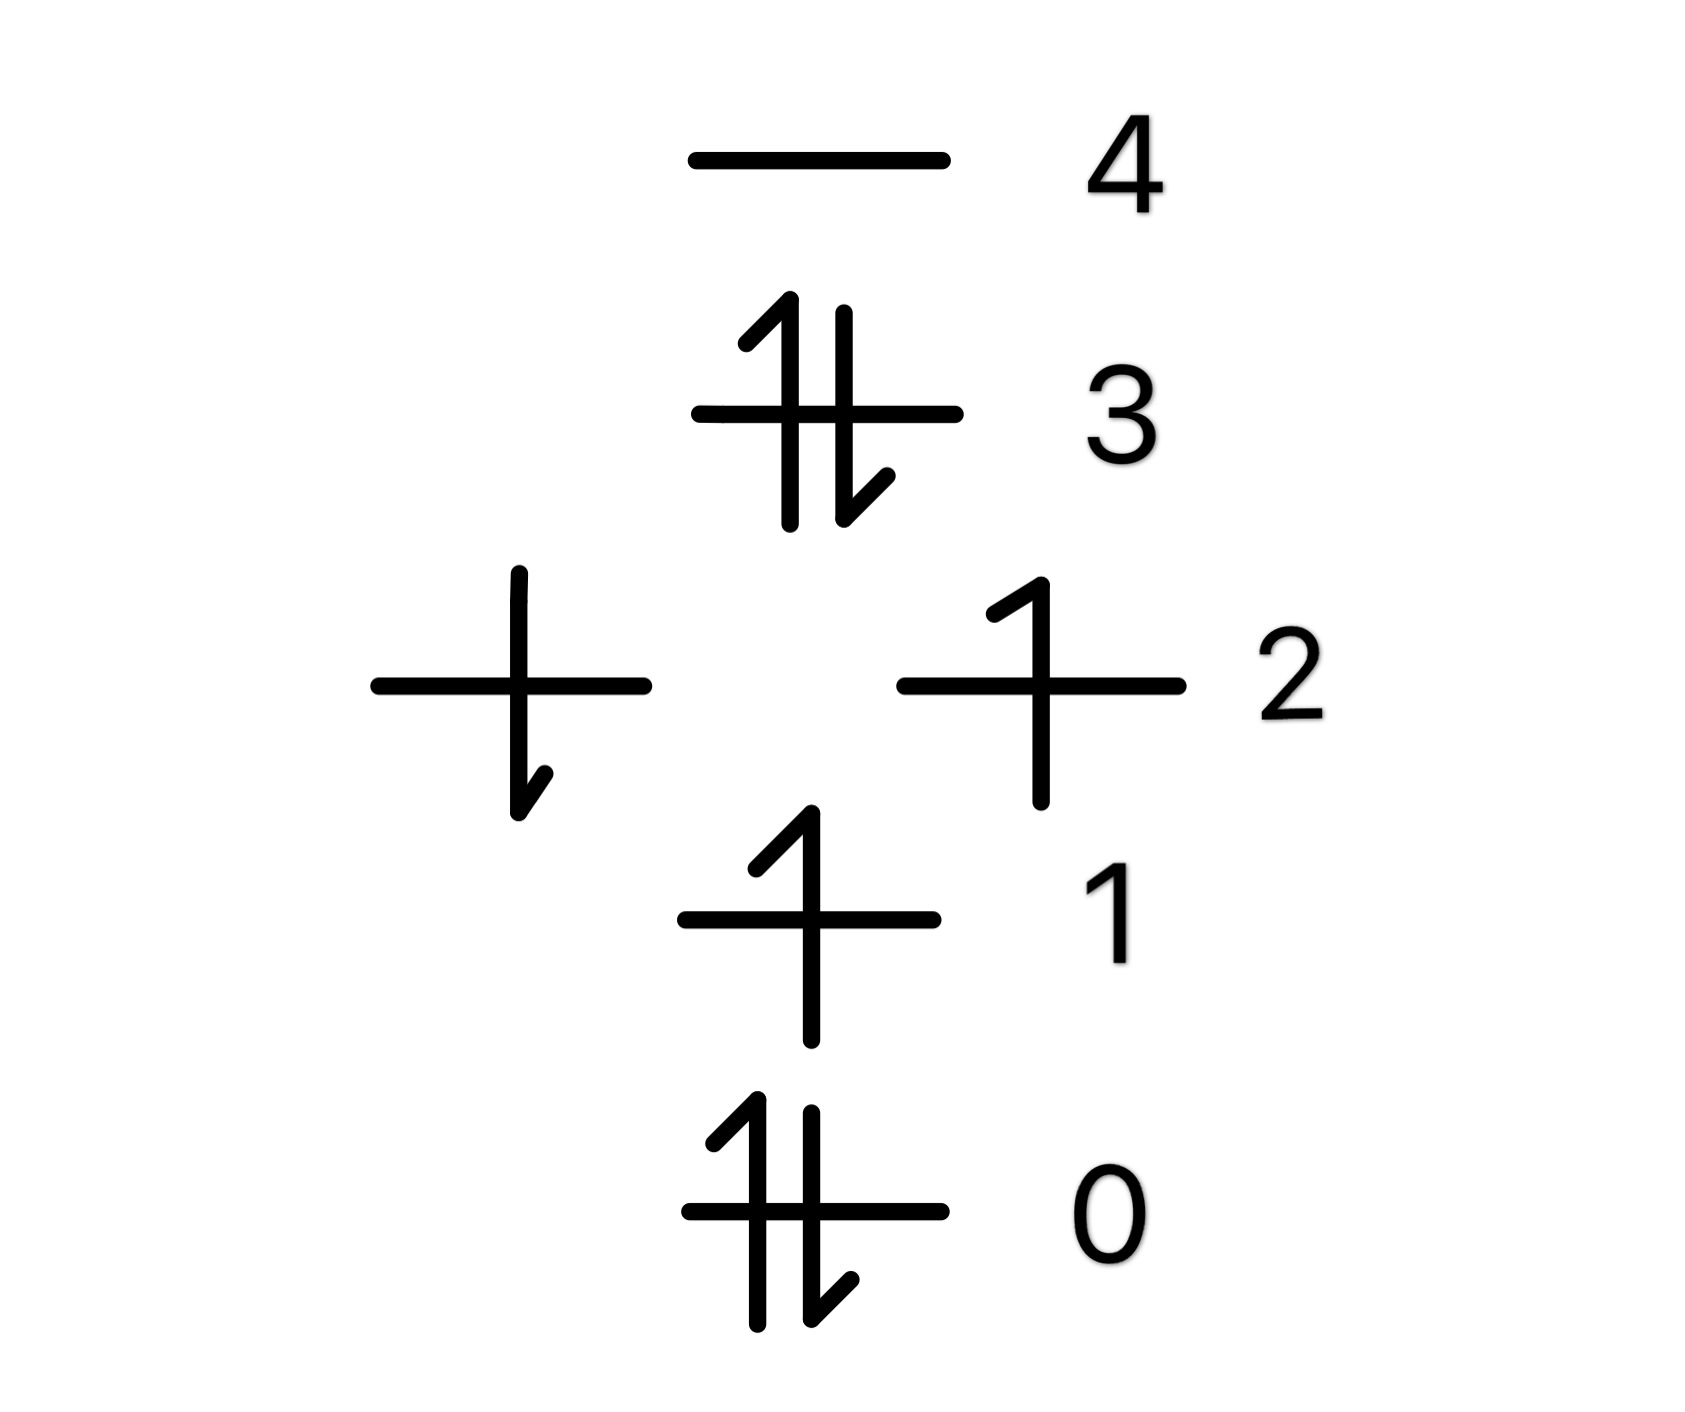
\includegraphics[width=5cm]{09.JPG}
\end{figure}\\
\tab Eigenstate of $\hat{h}$, eigenvalue: $2\varepsilon_0+\varepsilon_1+2\varepsilon_2+2\varepsilon_3$.\\
\tab For the wavefunctions of occupied orbital $\psi_{\lambda}$, the energy would be $E_{\lambda}=\sum_{i\in \lambda} \varepsilon_i$. (Limit to one spin-orbital per level)\\
\tab With this empirical rule (Pauli principle), we can understand orbital level structure of atoms and molecule. 
\paragraph{Spin} ~\\
\tab Orbitals also depend on spin. The easiest way to define is that orbitals are either of $\alpha$- or $\beta$- type. This indicates the eigenvalues of $\hat{s}_Z$ operator as $\frac{1}{2}, -\frac{1}{2}$.
\begin{IEEEeqnarray}{rLl} 
\hat{s}_Z(\alpha)&=\frac{1}{2}|\alpha\rangle  \\
\hat{s}_Z(\beta)&=-\frac{1}{2}|\beta\rangle \quad (\hbar=1)  
\end{IEEEeqnarray}
\tab ``Spin-orbitals":
\begin{IEEEeqnarray}{rLl} 
&\psi_a\alpha, \psi_a\beta, \psi_b\alpha, \psi_b\beta, \cdots \text{or} \\
&\psi_a, \bar{\psi}_a, \psi_b, \bar{\psi}_b, \cdots   
\end{IEEEeqnarray}
\tab NOTE: overbar labels $\beta$ spin.\\
\tab Consider product functions: 
\begin{IEEEeqnarray}{rLl} 
\psi_a(1)\bar{\psi}_a(2)\psi_b(3)\bar{\psi}_b(4) \cdots   
\end{IEEEeqnarray}
\tab Spin can be introduced in multiple ways. The above is easy, but does not incorporate many features. We will have a complete discussion later.\\
\tab The additional postulate is that a wavefunction for electrons has to change sign under interchange of a pair of electron labels.
\begin{IEEEeqnarray}{rLl} 
\psi(1,2,3,4) &= -\psi(2,1,3,4)  \notag \\
&= -\psi(1,2,4,3)\notag \\
&= +\psi(2,1,4,3)\notag \\
&= +\psi(2,3,1,4) \qquad \text{etc.} 
\end{IEEEeqnarray}
\tab For a product function this can be incorporated as antisymmetrizing the product. (spin-orbitals)
\tab Permutation in two electrons: 
\begin{IEEEeqnarray}{rLl} 
\hat{A}(\psi_a(1)\psi_b(2)) = \psi_a(1)\psi_b(2)- \psi_a(2)\psi_b(1) 
\end{IEEEeqnarray}
\tab Permutation in three electrons: 
\begin{IEEEeqnarray}{rLl} 
\hat{A}(\psi_a(1) \psi_b(2)\psi_c(3)) &= +\psi_a(1)\psi_b(2)\psi_c(3) \notag \\
&=-\psi_a(2)\psi_b(1)\psi_c(3) \notag \\
&=-\psi_a(3)\psi_b(2)\psi_c(1) \notag \\
&=-\psi_a(1)\psi_b(3)\psi_c(2) \notag \\
&=+\psi_a(3)\psi_b(1)\psi_c(2) \notag \\
&=+\psi_a(2)\psi_b(3)\psi_c(1)  \\
\notag \\
\hat{A}&= \sum_{i=1}^{N!} (-)^{p_i}\hat{P}_i	
\end{IEEEeqnarray}
\indent NOTE: \\
\tab \tab $\hat{A}$ represents antisymmetrization operator.\\
\tab \tab $p_i$ is called the parity of the permutation (0 or 1).\\
\tab \tab $N!$ is the total number of permutation of N electrons.\\
\tab \tab (+) sign: even number of interchanges\\
\tab \tab ($-$) sign: odd number of interchanges.\\

 It can verify that each of the terms have the same energy eigenvalues in many-electron system.
\begin{IEEEeqnarray}{rLl} 
E &= \varepsilon_a + \varepsilon_b +\cdots + \varepsilon_Z
\end{IEEEeqnarray}
\tab Because $\hat{h}(1)=\hat{h}(2)=\cdots=\hat{h}(N)$. $\hat{h}$ is symmetric in electrons, $\hat{A}\hat{h}-\hat{h}\hat{A}=0$
\begin{IEEEeqnarray}{rLl} 
&\sum_i\hat{h}(i)\hat{A}(\psi_a(1)\cdots\psi_Z(N) ) \notag \\
&=\hat{A}(\sum_i\hat{h}(i)\psi_a(1)\cdots\psi_Z(N) ) \notag \\
&=\hat{A}[(\varepsilon_a + \varepsilon_b +\cdots + \varepsilon_Z)(\psi_a(1)\cdots\psi_Z(N)) ] \notag \\
&=E\hat{A}(\psi_a(1)\cdots\psi_Z(N)) 
\end{IEEEeqnarray}
\tab The antisymmetrized product can be thought of in another (fully equivalent) way. Only wavefunctions that are allowed for electrons (Fermions) are antisymmetric.

\paragraph{Slater Determinant}~\\
\tab The antisymmetric wave function can be written as determinant and is called a Slater determinant. Also, the Slater determinant only works for product $\psi_a(1)\psi_b(2)\cdots$.
\begin{IEEEeqnarray}{rLl} 
\begin{vmatrix}
\psi_a(1) & \psi_a(2) \\
\psi_b(1) & \psi_b(2)	
\end{vmatrix} &= \psi_a(1)\psi_b(2) - \psi_a(2)\psi_b(1) \\
\notag \\
\begin{vmatrix}
\psi_a(1) & \psi_a(2) & \psi_a(3) \\
\psi_b(1) & \psi_b(2) & \psi_b(3) \\
\psi_c(1) & \psi_c(2) & \psi_c(3) 
\end{vmatrix} &= \psi_a(1)(\psi_b(2)\psi_c(3)-\psi_b(3)\psi_c(2)) \notag\\
& -\psi_b(1)(\psi_a(2)\psi_c(3)-\psi_a(3)\psi_c(2)) 	\notag\\
& +\psi_c(1)(\psi_a(2)\psi_b(3)-\psi_a(3)\psi_b(2))	
\end{IEEEeqnarray}
\tab From determinant picture it is easy to see that interchanges of electron labels, interchanges two columns.$\Longrightarrow$ change of sign.\\
\tab Solutions to Schr\"{o}dinger equation can be expressed as linear combinations of Slater determinants (antisymmetrized products). Energy is sum of orbital energies.\\
\tab In Slater determinant, every spin-orbital can at most be occupied once.However, the Slater determinant is analogous of product function. (very special, restrictive)
\\
\tab Pauli principle is a consequence of antisymmetry requirement.(undergrad chemistry of antisymmetry).
\begin{summary}{}{}
After consideration of antisymmetry of spin we can solve the one-electron problem:
    \begin{itemize}
    	\item  Solve one electron S.E: $\hat{h}\psi_a(1) = \sum_a \psi_a(1)$  (spatial orbitals)
    	\item Define spin orbitals $|\psi_a(1)\alpha \rangle|\psi_a(1)\beta \rangle = |\psi_a\rangle |\bar{\psi}_a \rangle$
    	\item Define N-electron Slater determinants. pick N distinct spin orbitals:\\ $|\psi_{\lambda}\rangle = |\psi_a(1)\psi_b(2)\cdots\psi_Z(N)\rangle$, $a<b<c<\cdots<Z$
    \end{itemize}
   
\end{summary}











\end{document}
